\documentclass[dvisvgm,border=2pt]{standalone}
% Shared by every figure. Two colours only: black becomes the text colour of
% whatever theme the app is in, and `accent` becomes the brand — see
% scripts/build-figures.mjs. Everything else is done with opacity.
\usepackage{amsmath}
\usepackage{amssymb}
\usepackage{tikz}
\usepackage{pgfplots}
\pgfplotsset{compat=1.18}
\usetikzlibrary{arrows.meta,positioning,calc,backgrounds,fit,patterns.meta}
\definecolor{accent}{RGB}{255,0,255}
\pgfplotsset{
  every axis/.append style={
    axis lines=left,
    axis line style={draw opacity=0.35},
    tick style={draw opacity=0.35},
    tick label style={font=\scriptsize,opacity=0.7},
    label style={font=\scriptsize,opacity=0.7},
    legend style={draw=none,fill=none,font=\scriptsize},
    every axis plot/.append style={line width=0.7pt},
  },
}
\tikzset{
  every picture/.style={font=\scriptsize},
  faint/.style={opacity=0.3},
  quiet/.style={opacity=0.55},
  box/.style={draw,opacity=0.35,rounded corners=2pt,inner sep=4pt},
  hot/.style={accent},
}

\begin{document}
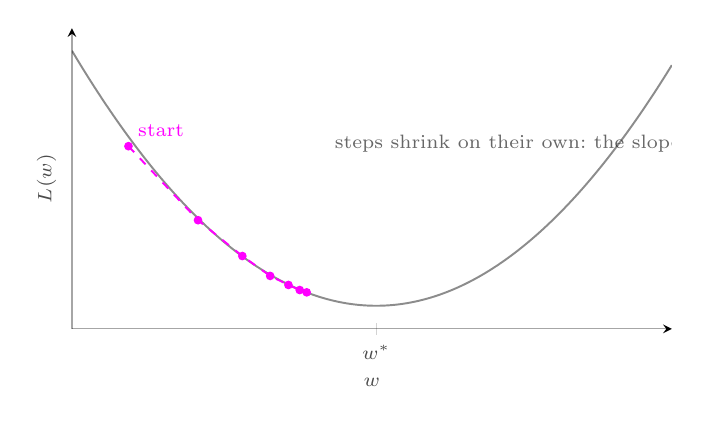
\begin{tikzpicture}
  \begin{axis}[width=9.2cm,height=5.4cm,
      xlabel={$w$},ylabel={$L(w)$},
      xmin=-0.3,xmax=6.6,ymin=0,ymax=13,
      ytick=\empty,xtick={3.2},xticklabels={$w^{*}$}]
    \addplot[domain=-0.3:6.6,samples=200,opacity=0.45]{0.9*(x-3.2)^2+1};
    % w <- w - eta L'(w), eta = 0.28, L' = 1.8 (w - 3.2)
    \addplot[accent,line width=0.7pt,dashed,mark=*,mark options={solid,accent,scale=0.6}]
      coordinates {(0.35,7.9)(1.15,4.7)(1.66,3.15)(1.98,2.29)(2.19,1.9)(2.32,1.68)(2.4,1.58)};
    \node[accent,anchor=south west,font=\scriptsize] at (axis cs:0.35,7.9) {start};
    \node[opacity=0.6,anchor=south,font=\scriptsize,align=center]
      at (axis cs:5.0,7.2) {steps shrink on their own:\ the slope does};
  \end{axis}
\end{tikzpicture}
\end{document}
